\documentclass[11pt,a4paper]{article}
\usepackage[margin=2.5cm]{geometry}
\usepackage[hidelinks]{hyperref}
\usepackage{graphicx}
\usepackage{booktabs}
\usepackage{amsmath}
\usepackage{enumitem}
\usepackage[T1]{fontenc}
\usepackage[utf8]{inputenc}
\usepackage{csquotes}
\usepackage{microtype}
\usepackage{array}
\usepackage{float}
\usepackage{bookmark}
\usepackage{tabularx}
\usepackage{pgfgantt}
\usepackage{rotating}
\usepackage{float}

\newcolumntype{L}{>{\raggedright\arraybackslash}X}
\setlist[itemize]{noitemsep,topsep=2pt}
\setlist[enumerate]{noitemsep,topsep=2pt}

% For pipeline visualization
\usepackage{tikz}
\usetikzlibrary{arrows.meta,positioning}

\title{Trust Analysis of Traffic Sign Classifiers under Uncertainties\\[2mm]
Bachelor Thesis Proposal}
\author{Youssef Hesham}
\date{\today}

\begin{document}
\maketitle

\section{Motivation}
\subsection{Research field}
Perception for intelligent vehicles combines real-time detection, tracking, and classification to interpret traffic scenes and support Advanced Driver Assistance Systems and autonomous driving. Traffic Sign Recognition (TSR) is a core capability: the system must localize signs in full-frame images and classify them into semantic categories whose meanings carry legal and safety consequences. Because high-confidence errors—such as misclassifying a Stop sign as a Priority road—may propagate to planning and control, TSR must be treated as safety-critical.

In real traffic, perception operates under severe uncertainty. Inputs vary with illumination, weather, motion blur, and sensor noise. However, uncertainty is not uniform; it is commonly divided into \textit{aleatoric} and \textit{epistemic} components, which require different handling.

\textbf{Aleatoric uncertainty} is inherent to the data observation itself and cannot be reduced by adding more training data. A practical example is found in datasets like \textit{Synset-Signset-Ger} \cite{synset2024}, where inherent design variations or severe degradations make certain examples not perfectly distinguishable even to a human observer. Whether due to motion blur or low resolution, this ambiguity is a property of the environment.

\textbf{Epistemic uncertainty}, conversely, reflects the model's lack of knowledge about regions of the input space it has not encountered during training. A critical example in TSR is physical-world sticker occlusions \cite{bayzidi2022stickers}. A stop sign covered by an arbitrary sticker may look unlike anything in the training set. Since ``every type of sticker could be possible,'' the model should ideally report high epistemic uncertainty (``I don't know'') rather than confidently misclassifying it.

Modern TSR systems use convolutional backbones such as ResNet variants and efficient one-stage detectors. While these models can reach high top-1 accuracy on curated datasets like GTSRB, their predicted probabilities often fail to reflect the true likelihood of correctness when facing these uncertainties. Trustworthy TSR therefore requires calibrated confidence and mechanisms to act on uncertainty, such as abstaining from prediction when confidence is low.

\begin{figure}[!htbp]
  \centering
  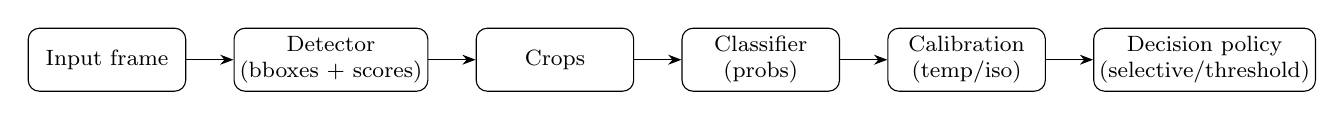
\begin{tikzpicture}[
    node distance=6mm,
    >=Stealth,
    block/.style={draw, rounded corners, align=center, minimum width=2.0cm, minimum height=8mm, inner sep=2pt},
    font=\footnotesize
  ]
    \node[block] (img) {Input frame};
    \node[block, right=of img] (det) {Detector\\(bboxes + scores)};
    \node[block, right=of det] (crop) {Crops};
    \node[block, right=of crop] (cls) {Classifier\\(probs)};
    \node[block, right=of cls] (cal) {Calibration\\(temp/iso)};
    \node[block, right=of cal] (policy) {Decision policy\\(selective/threshold)};
    \draw[->] (img) -- (det);
    \draw[->] (det) -- (crop);
    \draw[->] (crop) -- (cls);
    \draw[->] (cls) -- (cal);
    \draw[->] (cal) -- (policy);
  \end{tikzpicture}
  \caption{End-to-end TSR pipeline and where uncertainty, calibration, and selection are applied.}
  \label{fig:tsr-pipeline}
\end{figure}

Evaluation must reflect deployment. Rather than reporting only clean-set accuracy, robust assessment exposes models to controlled uncertainty sources. Because TSR classes can be visually similar (for example, speed-limit signs), small degradations can disproportionately harm calibration even when accuracy declines modestly. Finally, trustworthy TSR is a pipeline problem. Understanding how uncertainty propagates from detector to classifier—and designing simple, fast interventions—is central to deploying TSR that remains reliable when conditions are less than ideal.

\subsection{Thesis area}

This thesis analyzes and improves the trustworthiness of traffic sign classifiers under uncertainties within a real-time detection+classification pipeline. Using GTSRB \cite{stallkamp2011gtsrb} as the primary training benchmark, the work will rigorously evaluate performance against three distinct uncertainty categories:
\begin{enumerate}
    \item \textbf{Synthetic Aleatoric:} Controlled noise, blur, weather effects, and compression.
    \item \textbf{Epistemic Domain Shift:} Evaluation on the European Traffic Sign Dataset (ESD) \cite{gamez2018esd} to test generalization.
    \item \textbf{Physical Robustness:} Evaluation on the Sticker Occlusion dataset \cite{bayzidi2022stickers} to test resilience against adversarial-like attacks.
\end{enumerate}

The study will train ResNet-based classifiers \cite{he2016deep} in PyTorch as baselines and evaluate them with reliability diagrams, Expected Calibration Error (ECE), Brier score, and Negative Log-Likelihood (NLL) \cite{guo2017calibration, niculescu2005predicting}. Lightweight improvements will be prioritized: post-hoc calibration (temperature scaling and isotonic regression \cite{guo2017calibration}), single-pass confidence proxies (maximum probability, entropy, energy \cite{liu2020energy}), and Evidence-based Subjective Logic \cite{sensoy2018evidential}.

Where compute permits, budget-aware variants such as Monte-Carlo dropout \cite{gal2016dropout} or compact ensembles \cite{lakshminarayanan2017simple} may be included to compare trust-per-millisecond trade-offs. The outcome will be a reproducible pipeline and practical recommendations for deploying TSR that remains reliable when inputs are imperfect, all while staying within real-time limits.

\section{State of the Art}

Traffic Sign Recognition (TSR) in practice is a two-stage process: a real-time detector proposes candidate regions in the full image, and a classifier assigns a semantic label to each crop. Lightweight one-stage detectors (modern YOLO variants) are favored on embedded hardware, while ResNet-style CNN backbones remain strong baselines for classification \cite{stallkamp2011gtsrb,he2016deep,redmon2018yolov3}. Recent image backbones such as ConvNeXt and transformer-based architectures like Swin Transformer further improve accuracy–efficiency trade-offs on general vision tasks and are relevant for TSR \cite{liu2022convnext,liu2021swin}. On curated datasets such as GTSRB, clean, centered crops can yield high top-1 accuracy \cite{stallkamp2011gtsrb}.

However, deployment settings introduce multiple sources of uncertainty: sensor noise, motion blur, adverse weather, compression artifacts, illumination changes, partial occlusions, crop jitter from imperfect detections, and domain shifts across cameras or regions. Under these conditions, confidence estimates often become unreliable: models may be confidently wrong, undermining downstream safety logic \cite{ovadia2019can,minderer2021revisiting}. Furthermore, recent surveys on adversarial robustness indicate that while attacks are well-documented, practical mitigation strategies—specifically those viable for real-time systems—remain significantly underexplored \cite{pavlitska2023attacks}.

A large body of work addresses probability calibration. Post-hoc methods such as temperature scaling and isotonic regression adjust the final scores using a held-out calibration set and add essentially no runtime overhead \cite{guo2017calibration,niculescu2005predicting}. Training-time techniques (e.g., label smoothing or mixup) can influence calibration as well, but their effects vary with dataset and model capacity \cite{minderer2021revisiting}. Diagnostics include reliability diagrams, Expected Calibration Error (ECE), Brier score, and Negative Log-Likelihood, all of which quantify how predicted probabilities align with empirical correctness \cite{niculescu2005predicting,guo2017calibration}.

Uncertainty estimation complements calibration by indicating how much a prediction should be trusted. Single-pass proxies such as maximum softmax probability and entropy are attractive for real-time operation because they introduce negligible latency. Multi-pass approaches—Monte-Carlo dropout, stochastic weight sampling (e.g., SWAG), or small deep ensembles—typically improve error–confidence alignment but increase inference time and memory \cite{gal2016dropout,maddox2019simple,lakshminarayanan2017simple}.

Beyond these statistical proxies, recent strategies employ Subjective Logic—implemented via Evidential Deep Learning—to explicitly model trust \cite{sensoy2018evidential}. Unlike standard probabilities that must sum to one, Subjective Logic assigns mass to belief, disbelief, and uncertainty (vacuity). This allows the system to differentiate between conflicting evidence (aleatoric) and a total lack of evidence (epistemic) in a single forward pass, providing a mathematically grounded framework for trust assessment without the latency of ensembles \cite{han2025uncertainty}.

Decision-making under uncertainty is often studied through selective prediction (classification with a reject option). By abstaining on low-confidence inputs, systems can reduce error at the cost of coverage; risk–coverage curves summarize these trade-offs \cite{geifman2019selectivenet}. Thresholds are typically set on a calibration set; lightweight conformal-style thresholds can provide coverage guarantees under mild assumptions \cite{vovk2005algorithmic}. In TSR, selective strategies are especially useful when classes are visually similar (e.g., speed limits) and degradations remove fine details needed for disambiguation.

End-to-end pipeline effects remain underexplored. Many studies evaluate classification on perfect GTSRB crops, which hides failures introduced by detection, such as small or off-center crops that erase critical digits. Detector confidence and non-maximum suppression (NMS) determine which regions are kept: NMS suppresses overlapping boxes based on their scores, so miscalibrated detector scores can remove informative proposals before classification \cite{neubeck2006nms}. Trust should therefore be measured across the full pipeline and reported alongside latency. Robustness studies based on corruption benchmarks show that accuracy and calibration can degrade substantially under common corruptions, highlighting the need for stress testing beyond clean data \cite{hendrycks2019imagenetc}.

Comparisons across uncertainty methods often do not normalize for computational cost. This is a critical oversight because \textbf{inference efficiency} is the key constraint in real-time TSR: an uncertainty estimate that is computationally too expensive to run within the vehicle's decision deadline (e.g., 30\,ms braking window) is effectively useless for safety, regardless of its statistical quality.

\subsubsection*{Key limitations in existing solutions}

\begin{itemize}
  \item Calibration is frequently evaluated only on clean data; behavior under realistic uncertainties (noise, blur, weather, compression) and distribution shifts is often neglected or yields poor results \cite{ovadia2019can, hendrycks2019imagenetc}.
  \item Deployment-friendly methods are undercompared; many state-of-the-art results rely on ensembles or numerous stochastic passes (MC Dropout) that exceed real-time budgets for embedded systems \cite{lakshminarayanan2017simple, gal2016dropout}.
  \item Selective prediction and simple, guaranteed thresholding are rarely assessed specifically for TSR with clear coverage–risk and latency trade-offs \cite{geifman2019selectivenet}.
  \item End-to-end trust (detector + classifier) is seldom analyzed; assumptions of perfect crops in benchmarks like GTSRB mask failure modes introduced upstream by detector jitter \cite{stallkamp2011gtsrb}.
  \item Reproducible stress testing on GTSRB lacks standardized multi-severity perturbations with calibration and timing reported together.
\end{itemize}

This thesis addresses these gaps by building a reproducible, real-time oriented evaluation that measures both performance and confidence quality under controlled uncertainties, compares lightweight improvements, and analyzes trust for the full detection+classification pipeline.

\section{Problem Statement}

\subsection{Thesis focus}

Despite strong accuracy on curated datasets, traffic sign recognition systems often produce overconfident errors once uncertainty is introduced by real-world conditions. In a detection+classification pipeline, uncertainty arises from sensor noise, motion blur, weather, compression, domain shift, imperfect detections (crop jitter, scale changes), small object size, and partial visibility. The central problem is that classifier confidences, which downstream components rely on, may no longer reflect true likelihoods of correctness, undermining safety and decision logic in real time.

This thesis addresses the problem by (i) quantifying how different uncertainty sources affect both performance and calibration in a realistic pipeline, and (ii) developing lightweight methods that restore trustworthy confidence without violating latency constraints.

The work will design and implement the following artifacts:
\begin{itemize}
  \item A reproducible PyTorch pipeline that integrates a lightweight detector with a ResNet-based classifier, including tools to inject controlled uncertainties (noise, blur, weather, compression, crop jitter, partial visibility) at multiple severities.
  \item A trust module that provides single-pass confidence measures (maximum probability, entropy, energy) and post-hoc calibration methods (temperature scaling, isotonic regression) with negligible overhead.
  \item Optional budget-aware uncertainty baselines (e.g., a small number of Monte-Carlo dropout passes or a compact ensemble) to study trust gains per unit of additional computational complexity (GFLOPs).
  \item A selective prediction component that sets abstention thresholds on a held-out calibration set to achieve target coverage with bounded risk; thresholds are chosen to be simple and deployable.
  \item An evaluation harness that computes accuracy, Negative Log-Likelihood, Brier score, Expected Calibration Error, reliability diagrams, risk–coverage curves, and end-to-end latency; results are reported per uncertainty type and severity.
\end{itemize}

Methodology and scope:
\begin{itemize}
  \item Dataset: GTSRB for classification; detector-generated crops and controlled crop perturbations emulate realistic upstream noise when ground-truth boxes are unavailable.
  \item Training: ResNet-18 baselines and ConvNeXt-Tiny candidates with standard augmentation and regularization; clean/occluded and corrupted evaluation splits.
  \item Uncertainty stress tests: additive noise, blur (motion/defocus), weather effects, compression, brightness/contrast changes, crop jitter, and partial visibility masks—each with multiple severities.
  \item Real-time constraint: profile detector+classifier inference; prioritize single-pass methods; treat multi-pass methods as optional comparisons with explicit latency budgets.
  \item Analysis: per-class and per-severity breakdowns, error–confidence alignment, and ablations on calibration set size, class imbalance, augmentation strength, and crop quality.
\end{itemize}

Expected outcome is a practical set of recommendations—calibration settings, confidence thresholds, and simple selection policies—that maintain trustworthy behavior under uncertainties while meeting real-time requirements.

\subsection{Research questions}

\begin{enumerate}[label=\arabic*.]
  \item Why do specific uncertainty sources (e.g., noise, blur, crop jitter, partial visibility) degrade calibration more than others in TSR?
  \item What are the accuracy, calibration (ECE, Brier, NLL), and reliability diagrams across uncertainty types and severities for ResNet-based baselines?
  \item How do post-hoc methods (temperature scaling, isotonic regression) and single-pass confidence proxies (max probability, entropy, energy) compare in risk--coverage trade-offs relative to their \textbf{computational cost (GFLOPs)}?
  \item Can simple abstention thresholds, fitted on a small calibration set, maintain target coverage with acceptable risk across uncertainty shifts?
  \item Given a fixed computational budget, what incremental benefit is obtained from small-budget stochastic methods (e.g., few-pass MC dropout or a compact ensemble), and is the gain justified relative to their cost?
  \item How sensitive are trust metrics to detector imperfections (crop tightness, off-center crops), and can post-hoc calibration compensate for such upstream errors?
\end{enumerate}

\section{Approach}

This thesis establishes a reproducible detection+classification pipeline to quantify and mitigate trust failures. The methodology extends beyond standard accuracy metrics by integrating specific uncertainty estimation techniques—including Evidence-based Subjective Logic—and stress-testing them on both synthetic and real-world out-of-distribution datasets.

\subsection{Pipeline and Tooling}
The pipeline is implemented using \textbf{PyTorch Lightning} to ensure structured, reproducible training loops, and \textbf{Optuna} for efficient hyperparameter optimization.
The core architecture consists of:
\begin{itemize}
    \item \textbf{Detector:} A state-of-the-art YOLO variant (e.g., YOLOv11) serves as the region proposal network. We will investigate variants utilizing attention mechanisms to improve proposal quality under occlusion.
    \item \textbf{Classifier:} \textbf{ResNet-18} serves as the baseline CNN. To evaluate modern architectural improvements, we will compare this against \textbf{ConvNeXt-Tiny} \cite{liu2022convnext}, analyzing whether modern isotropic architectures offer better inherent calibration than standard pyramidal CNNs.
    \item \textbf{Pipeline Strategy:} While end-to-end approaches exist, this thesis maintains a two-stage (Detection $\rightarrow$ Classification) split. This design choice allows for the granular analysis of uncertainty sources—specifically isolating whether "trust" is lost due to poor localization (Detector) or semantic confusion (Classifier).
\end{itemize}

\subsection{Datasets and Uncertainty Sources}
To ensure a rigorous and scientifically robust evaluation, this work employs a multi-source benchmarking strategy that spans diverse data distributions:
\begin{itemize}
  \item \textbf{Training Distribution:} The German Traffic Sign Recognition Benchmark (GTSRB) \cite{stallkamp2011gtsrb} serves as the primary dataset. A fixed subset is reserved for calibration and threshold tuning.
  \item \textbf{Domain Shift (Epistemic Uncertainty):} To evaluate model behavior on unseen variations, the system is tested on the \textbf{European Traffic Sign Dataset (ESD)} \cite{gamez2018esd}, which introduces domain shifts in sign design and environmental context.
  \item \textbf{Physical Robustness:} The \textbf{Sticker Occlusion Dataset} \cite{bayzidi2022stickers} is incorporated to analyze performance under physical adversarial attacks and partial visibility—scenarios where standard Softmax often fails to capture high uncertainty.
  \item \textbf{Synthetic Aleatoric Uncertainty:} A controlled ``stress suite'' injects parameterized corruptions: additive noise, motion/defocus blur, weather overlays (rain/fog), and JPEG compression. To ensure photorealism beyond simple overlays, we will employ compositing techniques (alpha blending, edge smoothing) inspired by robust benchmarks like CURE-TSD \cite{temel2020cure}.
  \item \textbf{Open-Set Recognition (OSR):} To address the ``unknown unknown'' problem critical for autonomous safety, we will extend the OOD evaluation using a ``junk class'' dataset (e.g., non-traffic imagery). This validates whether the Subjective Logic ``Vacuity'' metric correctly identifies totally irrelevant inputs as ``Unknown'' rather than forcing a high-confidence false classification.
\end{itemize}

\subsection{Trust and Calibration Methods}
The project compares lightweight single-pass methods against rigorous evidential approaches:
\begin{itemize}
  \item \textbf{Post-hoc Calibration:} Temperature scaling and isotonic regression are applied to align confidence scores with empirical accuracy.
  \item \textbf{Subjective Logic (Evidential Deep Learning):} An Evidence-based classification head is implemented following \cite{sensoy2018evidential}. Unlike standard Softmax, which forces probabilities to sum to 1, this method models class probabilities as a Dirichlet distribution.
Crucially, this allows the calculation of \textbf{Vacuity} (uncertainty mass). We will investigate using this Vacuity score as a trigger for the "Safety Fallback" policy—for example, if Vacuity is high on a speed limit sign, the system defaults to the lowest restrictive speed (e.g., 30\,km/h) rather than guessing the most likely class.
  \item \textbf{Single-pass Proxies:} Maximum Softmax Probability (MSP), Entropy, and Energy-based scores \cite{liu2020energy} serve as baseline confidence measures.
  \item \textbf{Qualitative Explainability (Grad-CAM):} To qualitatively validate trust scores, we will employ Gradient-weighted Class Activation Mapping (Grad-CAM). This allows us to visualize saliency maps, ensuring that high-confidence predictions are grounded in relevant semantic features (e.g., the digits of a speed limit) rather than background artifacts or context.
\end{itemize}

\subsection{Justification of Metrics}
The selected metrics are aligned with the research questions to quantify safety and reliability:
\begin{itemize}
  \item \textbf{Expected Calibration Error (ECE):} Measures the gap between predicted confidence and actual accuracy, serving as a primary indicator of safety reliability.
  \item \textbf{Brier Score:} A proper scoring rule that penalizes both calibration error and low refinement, offering a holistic view of probabilistic quality.
  \item \textbf{Risk-Coverage Curves:} These quantify the operational trade-off between the level of automation (coverage) and the acceptable error rate (risk), determining the practical viability of the system.
  \item \textbf{Trust-per-Millisecond:} Normalizes calibration gains by computational cost to ensure suitability for real-time embedded hardware.
\end{itemize}

\begin{table}[!htbp]
\centering
\small
\caption{Experiment Grid (Updated).}
\label{tab:exp-grid}
\begin{tabularx}{\linewidth}{@{} l L @{}}
\toprule
Parameter & Values \\
\midrule
Frameworks & PyTorch Lightning, Optuna \\
Datasets & GTSRB (Train/Test), ESD (OOD Test), Sticker Occlusions (Robustness) \\
Trust Methods & Softmax (Baseline), Temperature Scaling, Subjective Logic (Evidential) \\
Uncertainty Sources & Noise, Blur, Weather, Compression, Crop Jitter, Physical Stickers \\
\bottomrule
\end{tabularx}
\end{table}

\subsection{Evaluation Metrics and Justification}
To strictly quantify the ``trustworthiness'' of the pipeline and answer the proposed research questions, we employ the following metrics. Each is selected to address a specific aspect of safety or efficiency.

\paragraph{Expected Calibration Error (ECE).}
ECE is the primary metric for \textbf{Research Question 2} (calibration quality). It measures the gap between the system's confidence and its actual accuracy, serving as a direct proxy for safety risks (i.e., preventing confident but wrong predictions).

Given predicted class probabilities $\{p_{ik}\}$ and confidences $\mathrm{conf}(x_i) = \max_k p_{ik}$, we partition predictions into $M$ confidence bins $\{B_m\}_{m=1}^M$. Let $\mathrm{acc}(B_m)$ be the empirical accuracy and $\mathrm{conf}(B_m)$ the mean confidence within bin $m$. The ECE is defined as:
$$
\mathrm{ECE} = \sum_{m=1}^{M} \frac{|B_m|}{n} \left| \mathrm{acc}(B_m) - \mathrm{conf}(B_m) \right|.
$$

\paragraph{Brier Score.}
While ECE measures calibration, it does not account for the sharpness of the distribution. The Brier score is a proper scoring rule that penalizes both calibration error and low refinement, offering a holistic view of probabilistic quality required for \textbf{Research Question 2}. With one-hot labels $y_{ik}$ for $K$ classes:
$$
\mathrm{Brier} = \frac{1}{n} \sum_{i=1}^{n} \sum_{k=1}^{K} \left(p_{ik} - y_{ik}\right)^2.
$$

\paragraph{Severity-Weighted Error (SWE).}
Standard accuracy treats all misclassifications equally. However, in TSR, misclassifying a 30\,km/h sign as 120\,km/h is fatal, whereas misclassifying it as 20\,km/h is merely conservative.
To address this, we define a cost matrix $W_{ij}$ representing the safety penalty of predicting class $j$ when the ground truth is $i$.
$$
\mathrm{SWE} = \frac{1}{n} \sum_{k=1}^{n} W_{y_k, \hat{y}_k}
$$
This ensures the model is evaluated not just on "correctness," but on "safety consequences," rewarding models that—when uncertain—fail gracefully (e.g., predicting lower speed limits rather than higher ones).

\paragraph{Trust Per Efficiency (TPE).}
Measuring raw latency (milliseconds) is often noisy and hardware-dependent. To address \textbf{Research Question 3} regarding the trade-off between reliability and computational cost in a hardware-agnostic manner, we define Trust Per Efficiency.

Let $\Delta \mathrm{ECE} = \mathrm{ECE}_{\text{base}} - \mathrm{ECE}_{\text{method}}$ be the gain in calibration, and $\Delta \mathrm{GFLOPs}$ be the increase in floating-point operations required by the uncertainty method.
$$
\mathrm{TPE} = \frac{\Delta \mathrm{ECE}}{\max(\Delta \mathrm{GFLOPs}, \epsilon)}
$$
This metric strictly quantifies the "architectural cost" of trust, independent of the specific GPU used for inference.

\section{Planning}

\subsection{Own Background}

I have practical experience with Python, PyTorch, and probability/statistics, as well as foundational knowledge of linear algebra, calculus, and machine learning. I am comfortable with CNN training, data preprocessing, and basic experiment tracking and plotting in Jupyter/Matplotlib.

\subsection{Skills to acquire}
\begin{itemize}
  \item Lightweight conformal prediction for classification and coverage guarantees.
  \item Latency profiling and optimization on GPU/CPU; measurement hygiene for per-frame timing.
  \item Detector integration and crop quality analysis; NMS behavior and calibration.
  \item Advanced calibration variants (per-class vs. global temperature; isotonic pitfalls).
  \item Robustness test design (severity scales, reproducible corruption pipelines).
\end{itemize}

\subsection{Required Resources}

\textbf{Hardware}

\begin{itemize}
  \item 1 GPU with $\geq$ 8--12\,GB VRAM (e.g., RTX 3060/3070 or university server GPU) for training and evaluation.
  \item Multi-core CPU, 16--32\,GB RAM, and $\sim$20\,GB storage for datasets, checkpoints, and logs.
  \item Reliable backup/storage and internet access for package and model downloads.
\end{itemize}

\textbf{Software}

\begin{itemize}
  \item Linux, Python 3.10+, PyTorch and TorchVision.
  \item Data/augmentation: Albumentations or \texttt{imgaug}; metrics: scikit-learn; plotting: Matplotlib/Seaborn.
  \item Experiment tracking: TensorBoard or Weights \& Biases; profiling: \texttt{torch.profiler}.
  \item Pre-trained lightweight detector (public weights) for sign region proposals.
\end{itemize}

\textbf{Data and assets}

\begin{itemize}
  \item GTSRB (classification) with a held-out calibration split.
  \item Synthetic uncertainty components (noise, blur, weather overlays, compression) and crop-jitter tooling.
  \item Optional: public traffic-sign detector model and any auxiliary scripts for crop extraction.
\end{itemize}

\subsection{Work packages}

Dated timeline for 13 Apr 2026 -- 15 Aug 2026 (single-student, \(\approx\)13 h/week). Key milestones are marked in brackets.

\begin{enumerate}[label=\textbf{W\arabic*}, leftmargin=*]
  \item 13--19 Apr: Kickoff — finalize scope/RQs, set up repo/environment, download GTSRB, initial reading.
  \item 20--26 Apr: Project definition — confirm milestones and latency targets; refine proposal with supervisor; focused literature map. \textbf{[M1: Proposal confirmed]}
  \item 27 Apr--03 May: Research \& planning — choose toolchain (PyTorch), configs, CI; freeze splits incl.\ a held‑out calibration set.
  \item 04--10 May: Data handling — clean/verify GTSRB, EDA, class balance, preprocessing; document train/val/test/calibration protocol.
  \item 11--17 May: Baseline modeling — train ResNet‑18 on clean crops; implement accuracy, NLL, Brier, ECE, reliability diagrams. \textbf{[M2: Baseline ready]}
  \item 18--24 May: Model development — regularization/augmentation tuning; stabilize baseline; seed control and logging.
  \item 25--31 May: Uncertainty stress suite v1 — add noise/blur/weather/compression (multi‑severity); evaluate accuracy \& calibration drift.
  \item 01--07 Jun: Mid‑term review — present baseline + stress results; adjust plan/ablations with supervisor. \textbf{[M3: Mid‑term review]}
  \item 08--14 Jun: Detection realism — implement crop jitter; integrate a lightweight pre‑trained detector to generate crops; compare to perfect crops.
  \item 15--21 Jun: System integration — end‑to‑end pipeline; latency profiling; optimizations to maximize trust-efficiency (TPE) within the real-time budget. \textbf{[M4: Real‑time E2E achieved]}
  \item 22--28 Jun: Calibration \& trust — add temperature scaling \& isotonic regression; compare single‑pass proxies (max‑prob, entropy, energy); start selective prediction.
  \item 29 Jun--05 Jul: Ablations \& advanced tests — per‑class analyses; sensitivity to crop tightness/off‑center; optional few‑pass MC dropout or small ensemble if time allows. \textbf{[M5: Results freeze]}
  \item 06--12 Jul: Presentation preparation — finalize plots/tables; compile recommendations (thresholds, policies); draft slides and demo.
  \item 13--19 Jul: Writing block — methods, experiments, results; supervisor feedback round.
  \item 20--26 Jul: Wrap‑up draft — discussion, limitations, future work; polish figures; prepare artifact package (code/configs).
  \item 27 Jul--02 Aug: Buffer \& revisions — address feedback; dry‑run talk; finalize timings and demo assets.
  \item 03--09 Aug: Final presentation/defense window — deliver talk and demo; incorporate committee feedback. \textbf{[M6: Defense]}
  \item 10--15 Aug: Final wrap‑up — camera‑ready thesis; artifact release; checklist and submission. \textbf{[M7: Final submission]}
\end{enumerate}

\clearpage
\begin{sidewaysfigure}
\centering
    % We use x unit=1.5mm to ensure the total width is safe for LaTeX math
    % 125 days * 1.5mm = ~18cm, which fits perfectly on the page height
    \begin{ganttchart}[
        vgrid={*1{draw=black!20}},
        hgrid,
        time slot format=isodate,
        x unit=1.5mm, 
        time slot unit=day,
        calendar week text={W\currentweek},
        % Visual Styles
        bar/.append style={fill=blue!40, draw=blue!70, line width=1pt},
        bar height=0.6,
        bar label font=\bfseries\scriptsize, 
        group label font=\bfseries\small,
        milestone/.append style={fill=red, draw=red!80},
        milestone label font=\itshape\scriptsize,
        title/.style={draw=none, fill=none},
        title label font=\bfseries\tiny,
        y unit title=0.5cm,
        y unit chart=0.6cm
    ]{2026-04-13}{2026-08-15}
    
    % --- Calendar Header ---
    \gantttitlecalendar{year, month=name, week} \\
    
    % --- Phase 1 ---
    \ganttgroup{Phase 1: Setup \& Definition}{2026-04-13}{2026-05-03} \\
    \ganttbar{Kickoff \& Literature}{2026-04-13}{2026-04-19} \\
    \ganttbar{Refine Proposal}{2026-04-20}{2026-04-26} \\
    \ganttmilestone{M1: Proposal Confirmed}{2026-04-26} \\
    \ganttbar{Repo \& Splits Setup}{2026-04-27}{2026-05-03} \\
    
    % --- Phase 2 ---
    \ganttgroup{Phase 2: Baselines}{2026-05-04}{2026-05-31} \\
    \ganttbar{Data Cleaning/EDA}{2026-05-04}{2026-05-10} \\
    \ganttbar{Train ResNet Baseline}{2026-05-11}{2026-05-17} \\
    \ganttmilestone{M2: Baseline Ready}{2026-05-17} \\
    \ganttbar{Stress Suite (Noise/Blur)}{2026-05-25}{2026-05-31} \\
    
    % --- Phase 3 ---
    \ganttgroup{Phase 3: Integration}{2026-06-01}{2026-06-28} \\
    \ganttmilestone{M3: Mid-term Review}{2026-06-07} \\
    \ganttbar{Detector \& Crop Jitter}{2026-06-08}{2026-06-14} \\
    \ganttbar{Pipeline Integration}{2026-06-15}{2026-06-21} \\
    \ganttmilestone{M4: Real-time E2E}{2026-06-21} \\
    \ganttbar{Calibration \& Subj. Logic}{2026-06-22}{2026-06-28} \\
    
    % --- Phase 4 ---
    \ganttgroup{Phase 4: Eval \& Writing}{2026-06-29}{2026-08-15} \\
    \ganttbar{Ablations \& Analysis}{2026-06-29}{2026-07-05} \\
    \ganttmilestone{M5: Results Freeze}{2026-07-05} \\
    \ganttbar{Thesis Writing}{2026-07-13}{2026-08-02} \\
    \ganttmilestone{M6: Defense}{2026-08-09} \\
    \ganttmilestone{M7: Submission}{2026-08-15}
    
    \end{ganttchart}
    \caption{Project Timeline and Milestones}
    \label{fig:gantt}
\end{sidewaysfigure}
\clearpage

\subsection{Contingency plan}

\begin{itemize}
  \item \textbf{Risk:} Real-time budget is exceeded by multi-pass methods. \textbf{Mitigation:} Prioritize single-pass calibration and confidence proxies; keep MC dropout/ensembles optional and report trust gains normalized by latency.
  \item \textbf{Risk:} Calibration fails to generalize across uncertainty types. \textbf{Mitigation:} Compare global vs. per-class temperature, isotonic regression, and threshold recalibration per uncertainty family; use simple conformal-style thresholds to control coverage.
  \item \textbf{Risk:} Compute or time constraints limit experimentation. \textbf{Mitigation:} Freeze scope at single-pass methods and the most impactful uncertainties; reduce grid sizes; reuse pre-trained backbones.
  \item \textbf{Risk:} Results are hard to reproduce. \textbf{Mitigation:} Fixed seeds, config files, environment locking, and automated report generation; publish scripts and documentation.
  \item \textbf{Risk:} Generated synthetic occlusions lack physical realism. \textbf{Mitigation:} Adopt proven blending methodologies (e.g., CURE-TSD) and leverage high-quality occlusion mask libraries from concurrent research groups to ensure diversity in vegetation and obstacle patterns.
\end{itemize}

\begin{thebibliography}{99}

% --- Original Baselines ---
\bibitem{stallkamp2011gtsrb}
J.~Stallkamp, M.~Schlipsing, J.~Salmen, and C.~Igel,
\newblock ``The German Traffic Sign Recognition Benchmark: A multi-class classification competition,''
\newblock In \emph{Proc. IJCNN}, 2011.

\bibitem{he2016deep}
K.~He, X.~Zhang, S.~Ren, and J.~Sun,
\newblock ``Deep Residual Learning for Image Recognition,''
\newblock In \emph{Proc. CVPR}, 2016.

% --- The "Subjective Logic" & Trust Papers (Requested by Supervisor) ---
\bibitem{sensoy2018evidential}
M.~Sensoy, L.~Kaplan, and M.~Kandemir,
\newblock ``Evidential Deep Learning to Quantify Classification Uncertainty,''
\newblock In \emph{Proc. NeurIPS}, 2018.

\bibitem{han2025uncertainty}
Z.~Han, et al.,
\newblock ``Deep-Learning-Based Uncertainty-Estimation Approach for Unknown Traffic Identification,''
\newblock \emph{IEEE Intelligent Systems}, 2025.

% --- The "Sticker/Occlusion" Paper (Requested by Supervisor) ---
\bibitem{bayzidi2022stickers}
Y.~Bayzidi, A.~Smajic, F.~H{\"u}ger, R.~Moritz, S.~Varghese, P.~Schlicht, and A.~Knoll,
\newblock ``Traffic Sign Classifiers Under Physical World Realistic Sticker Occlusions: A Cross Analysis Study,''
\newblock In \emph{Proc. IEEE Intelligent Vehicles Symposium (IV)}, pp. 644--650, 2022.

% --- The "European Traffic Signs" Dataset (Requested by Supervisor) ---
\bibitem{gamez2018esd}
C.~G{\'a}mez-Serna and Y.~Ruichek,
\newblock ``Classification of Traffic Signs: The European Dataset,''
\newblock \emph{IEEE Access}, 2018.

% --- New State of the Art (2022-2025) ---
\bibitem{gawlikowski2023survey}
J.~Gawlikowski, et al.,
\newblock ``A Survey of Uncertainty in Deep Neural Networks,''
\newblock \emph{Artificial Intelligence Review}, vol. 56, 2023.

\bibitem{krizhevsky2024yolo}
A.~Kozhamkulova, et al.,
\newblock ``Development of Deep Learning Models for Traffic Sign Recognition in Autonomous Vehicles,''
\newblock \emph{International Journal of Advanced Computer Science and Applications}, vol. 15, no. 5, 2024.

\bibitem{bhatt2024yolov11}
A.~Bhatt,
\newblock ``Performance Comparison in Traffic Sign Recognition Using Deep Learning (YOLOv11),''
\newblock \emph{ResearchGate Preprint}, 2024.

% --- Existing Citations ---
\bibitem{liu2022convnext}
Z.~Liu, H.~Mao, C.-Y.~Wu, C.~Feichtenhofer, T.~Darrell, and S.~Xie,
\newblock ``A ConvNet for the 2020s,''
\newblock In \emph{Proc. CVPR}, 2022.

\bibitem{liu2021swin}
Z.~Liu, Y.~Lin, Y.~Cao, H.~Hu, Y.~Wei, Z.~Zhang, S.~Lin, and B.~Guo,
\newblock ``Swin Transformer: Hierarchical Vision Transformer using Shifted Windows,''
\newblock In \emph{Proc. ICCV}, 2021.

\bibitem{neubeck2006nms}
A.~Neubeck and L.~Van Gool,
\newblock ``Efficient Non-Maximum Suppression,''
\newblock In \emph{Proc. ICPR}, 2006.

\bibitem{redmon2018yolov3}
J.~Redmon and A.~Farhadi,
\newblock ``YOLOv3: An Incremental Improvement,''
\newblock \emph{arXiv:1804.02767}, 2018.

\bibitem{guo2017calibration}
C.~Guo, G.~Pleiss, Y.~Sun, and K.~Q. Weinberger,
\newblock ``On Calibration of Modern Neural Networks,''
\newblock In \emph{Proc. ICML}, 2017.

\bibitem{niculescu2005predicting}
A.~Niculescu-Mizil and R.~Caruana,
\newblock ``Predicting Good Probabilities with Supervised Learning,''
\newblock In \emph{Proc. ICML}, 2005.

\bibitem{vovk2005algorithmic}
V.~Vovk, A.~Gammerman, and G.~Shafer,
\newblock \emph{Algorithmic Learning in a Random World},
\newblock Springer, 2005.

\bibitem{hendrycks2019imagenetc}
D.~Hendrycks and T.~Dietterich,
\newblock ``Benchmarking Neural Network Robustness to Common Corruptions and Perturbations,''
\newblock In \emph{Proc. ICLR}, 2019.

\bibitem{gal2016dropout}
Y.~Gal and Z.~Ghahramani,
\newblock ``Dropout as a Bayesian Approximation: Representing Model Uncertainty in Deep Learning,''
\newblock In \emph{Proc. ICML}, 2016.

\bibitem{lakshminarayanan2017simple}
B.~Lakshminarayanan, A.~Pritzel, and C.~Blundell,
\newblock ``Simple and Scalable Predictive Uncertainty Estimation using Deep Ensembles,''
\newblock In \emph{Proc. NeurIPS}, 2017.

\bibitem{geifman2019selectivenet}
Y.~Geifman and R.~El-Yaniv,
\newblock ``SelectiveNet: A Deep Neural Network with an Integrated Reject Option,''
\newblock In \emph{Proc. ICML}, 2019.

\bibitem{ovadia2019can}
Y.~Ovadia, et al.,
\newblock ``Can You Trust Your Model's Uncertainty? Evaluating Predictive Uncertainty under Dataset Shift,''
\newblock In \emph{Proc. NeurIPS}, 2019.

\bibitem{minderer2021revisiting}
M.~Minderer, et al.,
\newblock ``Revisiting the Calibration of Modern Neural Networks,''
\newblock In \emph{Proc. NeurIPS}, 2021.

\bibitem{liu2020energy}
W.~Liu, X.~Wang, J.~Owens, and Y.~Li,
\newblock ``Energy-based Out-of-Distribution Detection,''
\newblock In \emph{Proc. NeurIPS}, 2020.

\bibitem{maddox2019simple}
W.~J.~Maddox, et al.,
\newblock ``A Simple Baseline for Bayesian Uncertainty in Deep Learning,''
\newblock In \emph{Proc. NeurIPS}, 2019.

\bibitem{synset2024}
SynSet Project,
\newblock ``SynSet: Synthetic Datasets for Autonomous Driving,''
\newblock \url{https://synset.de/datasets/synset-signset-ger/}, Accessed: 2025.

\bibitem{pavlitska2023attacks}
S.~Pavlitska, N.~Lambing, and J.~M. Zöllner,
\newblock ``Adversarial attacks on traffic sign recognition: A survey,''
\newblock In \emph{Proc. ICECCME}, 2023.

\bibitem{temel2020cure}
D.~Temel, M.-H. Chen, and G. AlRegib,
\newblock ``Traffic Sign Detection Under Challenging Conditions: A Deeper Look Into Performance Variations,''
\newblock \emph{IEEE Transactions on Intelligent Transportation Systems}, 2020.

\end{thebibliography}

\end{document}